\documentclass{article}
\usepackage[utf8]{inputenc}    % For UTF-8 character encoding
\usepackage[T1]{fontenc}       % For proper font encoding
\usepackage{lmodern}           % Improved font rendering
\usepackage{amsmath}   % For advanced mathematical formatting
\usepackage{amssymb}   % For mathematical symbols
\usepackage{geometry}  % Adjust page margins
\usepackage{enumerate} % For custom lists
\usepackage{xcolor}  % for coloring
\usepackage{amsthm}
\usepackage{pdfpages}
\newtheorem{theorem}{Theorem}[section]
\newtheorem{lemma}[theorem]{Lemma}
\newtheorem{corollary}[theorem]{Corollary}
\newtheorem{definition}[theorem]{Definition}
\usepackage{listings}  % for code listings

\lstset{frame=tb,
  language=C,
  aboveskip=3mm,
  belowskip=3mm,
  showstringspaces=false,   
  columns=flexible,
  basicstyle={\small\ttfamily},
  numbers=none,
  numberstyle=\tiny\color{gray},
  keywordstyle=\color{blue},
  commentstyle=\color{brown},
  stringstyle=\color{orange},
  breaklines=true,
  breakatwhitespace=true,
  tabsize=3
}
\geometry{top=1in, bottom=1in, left=1in, right=1in}

\begin{document}

\title{}
\author{Wang Xiyu}
\date{}
\maketitle
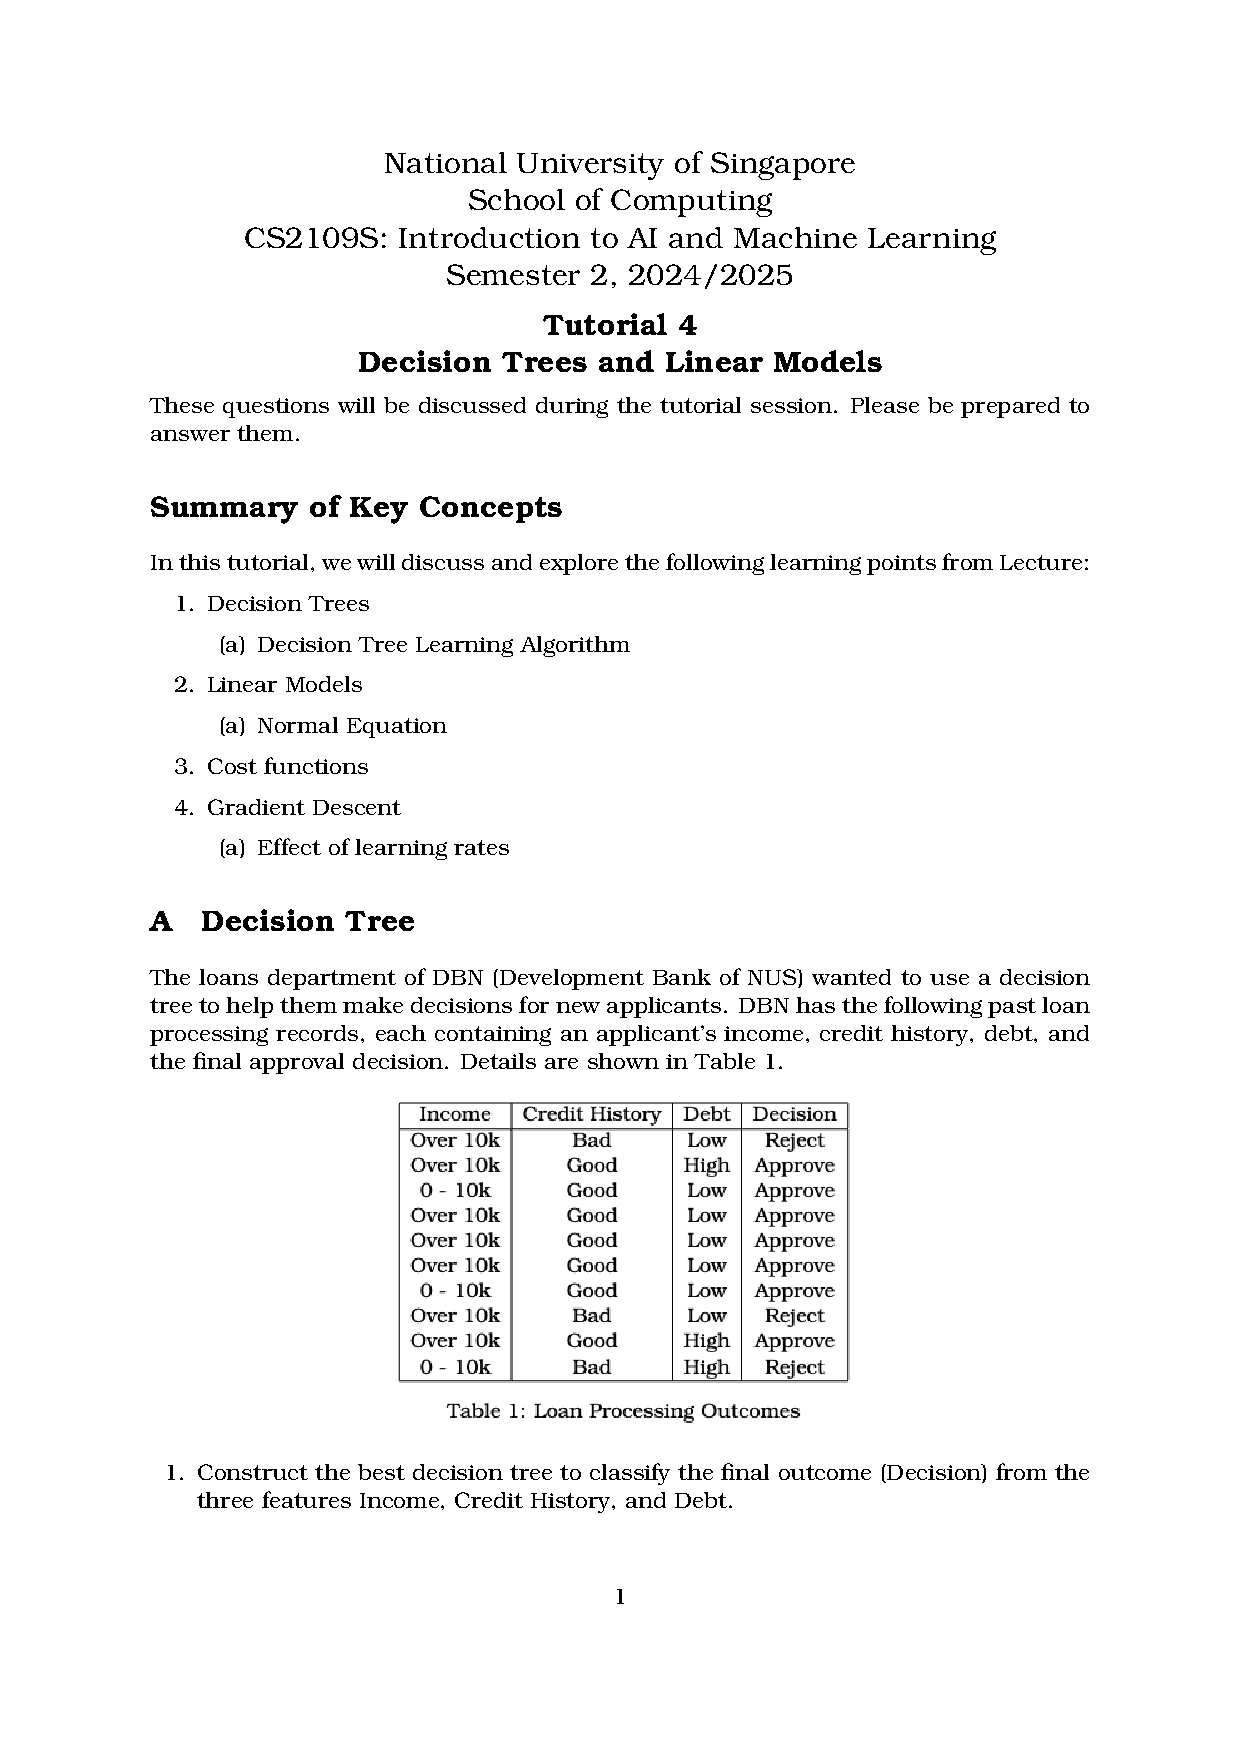
\includepdf[pages=1]{Tutorial4.pdf}
\section*{A}
\subsection*{Construct Decision Tree}
\begin{lstlisting}
  if (Credit History == Bad) -> Reject
  else -> accept
\end{lstlisting}

\subsection*{}
\begin{itemize}
  \item Income: 0 - 10k -> 0; Over 10k -> 1
  \item Credit History: Bad -> 0; Good -> 1
  \item Debt: High -> 0; Low -> 1
\end{itemize}

$IG(Income) = 1 - [\frac{3}{10}I(\frac{2}{3}, \frac{1}{3}) + \frac{7}{10}I(\frac{6}{7}, \frac{1}{7})] = 
1 - [-\frac{3}{10}(\frac{2}{3}log_2(\frac{2}{3}) - \frac{1}{3}log_2(\frac{1}{3})) + \frac{7}{10}(\frac{6}{7}log_2(\frac{6}{7})- \frac{1}{7}log_2(\frac{1}{7}))]
= 1 - [\frac{3}{10}(\frac{2}{3}(log_2(2) - log_2(3) - ))]$...

\subsection*{4}
\begin{itemize}
    \item More data
    \item add feature
    \item min sample pruning
    \item remove outliers
\end{itemize}
\subsection*{3}


\includepdf[pages=2]{Tutorial4.pdf}
\includepdf[pages=3]{Tutorial4.pdf}

\subsection*{1}
\[IG(A) = I(\frac{p}{p + n}, \frac{n}{p + n}) - remainder(A)\]
\[I(P(+), P(-)) = -\frac{p}{p + n}log_2 \frac{p}{p + n} - \frac{n}{p+n}log_2\frac{n}{p+n}\]

\[remainder(A) = \sum_{i=1}^{v}\frac{p_i + n_i}{p + n}I(\frac{p_i}{p_i + n_i}, \frac{n_i}{p_i + n_i})\]
\begin{lstlisting}
  import numpy as np
  def compute_Info_boolean(pos, neg):
      pos_prob = np.divide(pos, (pos + neg), dtype=np.float128)
      neg_prob = np.divide(neg, (pos + neg), dtype=np.float128)
      return - pos_prob * np.log2(pos_prob) - neg_prob * np.log2(neg_prob)
  
  def entropy(pos, neg):
      total = pos + neg
      if total == 0: 
          return 0
      pos_prob = np.divide(pos, total, dtype=np.float128)
      neg_prob = np.divide(neg, total, dtype=np.float128)
      entropy = 0
      if pos_prob > 0:
          entropy -= pos_prob * np.log2(pos_prob)
      if neg_prob > 0:
          entropy -= neg_prob * np.log2(neg_prob)
  
      return entropy
  
  def compute_IG_boolean(parent_pos, parent_neg, left_pos, left_neg, right_pos, right_neg):
      parent_entropy = entropy(parent_pos, parent_neg)
      total_parent = parent_pos + parent_neg
      total_left = left_pos + left_neg
      total_right = right_pos + right_neg
      left_weight = np.divide(total_left, total_parent, dtype=np.float128) if total_left > 0 else 0
      right_weight = np.divide(total_right, total_parent, dtype=np.float128) if total_right > 0 else 0
      weighted_child_entropy = left_weight * entropy(left_pos, left_neg) + right_weight * entropy(right_pos, right_neg)
      return parent_entropy - weighted_child_entropy
  
  
  
  x1 = np.matrix([[6], [8], [12], [2]])
  x2 = np.matrix([[4], [5], [9], [1]])
  x3 = np.matrix([[11], [9], [25], [3]])
  y = np.matrix([[20], [1], [3], [7]])
  X = np.hstack([x1, x2, x3])
  Xt = np.transpose(X)
  w = np.linalg.inv(Xt @ X) @ Xt @ y
  print(w)
  
\end{lstlisting}


\subsection*{2}
When $det(X^TX) = 0$, Linearly dependent column: Highly correlated features.
\subsubsection*{}
\begin{itemize}
    \item remove feature
    \item regularization
    \item pseudo invert
    \item use gradient descent
\end{itemize}
\section*{Normal Equation}
\noindent Derive:
\begin{equation}
  w = (X^T X)^{-1} X^T y.
\end{equation}
From:
\begin{equation}
    MSE = \frac{1}{N} \sum_{i=1}^{N}(\hat{y}^{(i)} - y^{(i)})^2 
\end{equation}

\section*{Proof}
We start with the Mean Squared Error (MSE) function:
\begin{equation}
    MSE = \frac{1}{N} \sum_{i=1}^{N} (\hat{y}^{(i)} - y^{(i)})^2,
\end{equation}
where \( \hat{y}^{(i)} = h_w(x^{(i)}) = w^T x^{(i)} \), with \( w \in \mathbb{R}^{d \times 1} \) and \( y \in \mathbb{R}^{N \times 1} \).
Expanding in terms of matrix notation, let \( A = Xw - y \), where \( X \in \mathbb{R}^{N \times d} \) with rows \( x^{(i)} \), then:
\begin{equation}
    MSE = \frac{1}{N} \sum_{i=1}^{N} (w^T x^{(i)} - y^{(i)})^2 = \frac{1}{N} (A^T A).
\end{equation}
Rewriting:
\begin{equation}
    MSE = \frac{1}{N} (Xw - y)^T (Xw - y),
\end{equation}
which expands further as:
\begin{equation}
    MSE = \frac{1}{N} \left( w^T X^T X w - w^T X^T y - y^T X w + y^T y \right).
\end{equation}
Since \( w^T X^T X w \) and \( y^T X w \) are scalars, we simplify:
\begin{equation}
    MSE = \frac{1}{N} \left( w^T X^T X w - 2 w^T X^T y + y^T y \right).
\end{equation}
To minimize MSE, we take the partial derivative with respect to \( w \):
\begin{equation}
    \frac{\partial}{\partial w} \left[ \frac{1}{N} \left( w^T X^T X w - 2 w^T X^T y + y^T y \right) \right].
\end{equation}
Differentiating term by term:
\begin{equation}
    \frac{\partial}{\partial w} (w^T X^T X w) = 2X^T X w,
\end{equation}
\begin{equation}
    \frac{\partial}{\partial w} (-2 w^T X^T y) = -2 X^T y,
\end{equation}
\begin{equation}
    \frac{\partial}{\partial w} (y^T y) = 0.
\end{equation}
Thus,
\begin{equation}
    \frac{\partial}{\partial w} (MSE) = \frac{1}{N} (2X^T X w - 2X^T y).
\end{equation}
Setting the derivative to zero for minimization:
\begin{equation}
    \frac{2}{N} X^T X w - \frac{2}{N} X^T y = 0.
\end{equation}
\begin{equation}
    X^T X w = X^T y.
\end{equation}
Solving for \( w \), assuming \( X^T X \) is invertible:
\begin{equation}
    w = (X^T X)^{-1} X^T y.
\end{equation}
\includepdf[pages=4]{Tutorial4.pdf}
\section*{B}
\subsection*{a}
\subsection*{}
To minimize the impact of outliers, use MAE it penalize the impact of outliers less
\subsection*{}

\includepdf[pages=5]{Tutorial4.pdf}




\section{}




\end{document}
